\documentclass[10pt]{article}
\usepackage[margin=0.75in]{geometry}
\usepackage{graphicx,booktabs,hyperref,amssymb}
\hypersetup{colorlinks=true,urlcolor=blue}
\title{Fast-Kummer model applicability on 21 transferred curves}
\author{Exact arithmetic gate}
\date{21 October 2026}
\begin{document}
\maketitle
\noindent\textbf{Scope.} The exact genus-2 quintics from the frozen 21-model
cohort were evaluated at every $x\in\mathbb F_p$. Every quintic had five
distinct roots in $\mathbb F_p$. For each model, the program also checked
the derivative at each root and reconstructed the original polynomial from
the five linear factors. The native output was reproduced byte-for-byte in
a separate run. Thus the six Weierstrass points, including infinity, are
rational on all 21 models, yielding full rational two-torsion.

\begin{center}
\begin{tabular}{lrr}
\toprule
Exact gate & Passing models & Checked models \\
\midrule
Five distinct finite rational roots & 21 & 21 \\
Polynomial reconstructed from roots & 21 & 21 \\
Unsigned ordinary-addition ambiguity witness & 21 & 21 \\
\bottomrule
\end{tabular}
\end{center}
\begin{center}
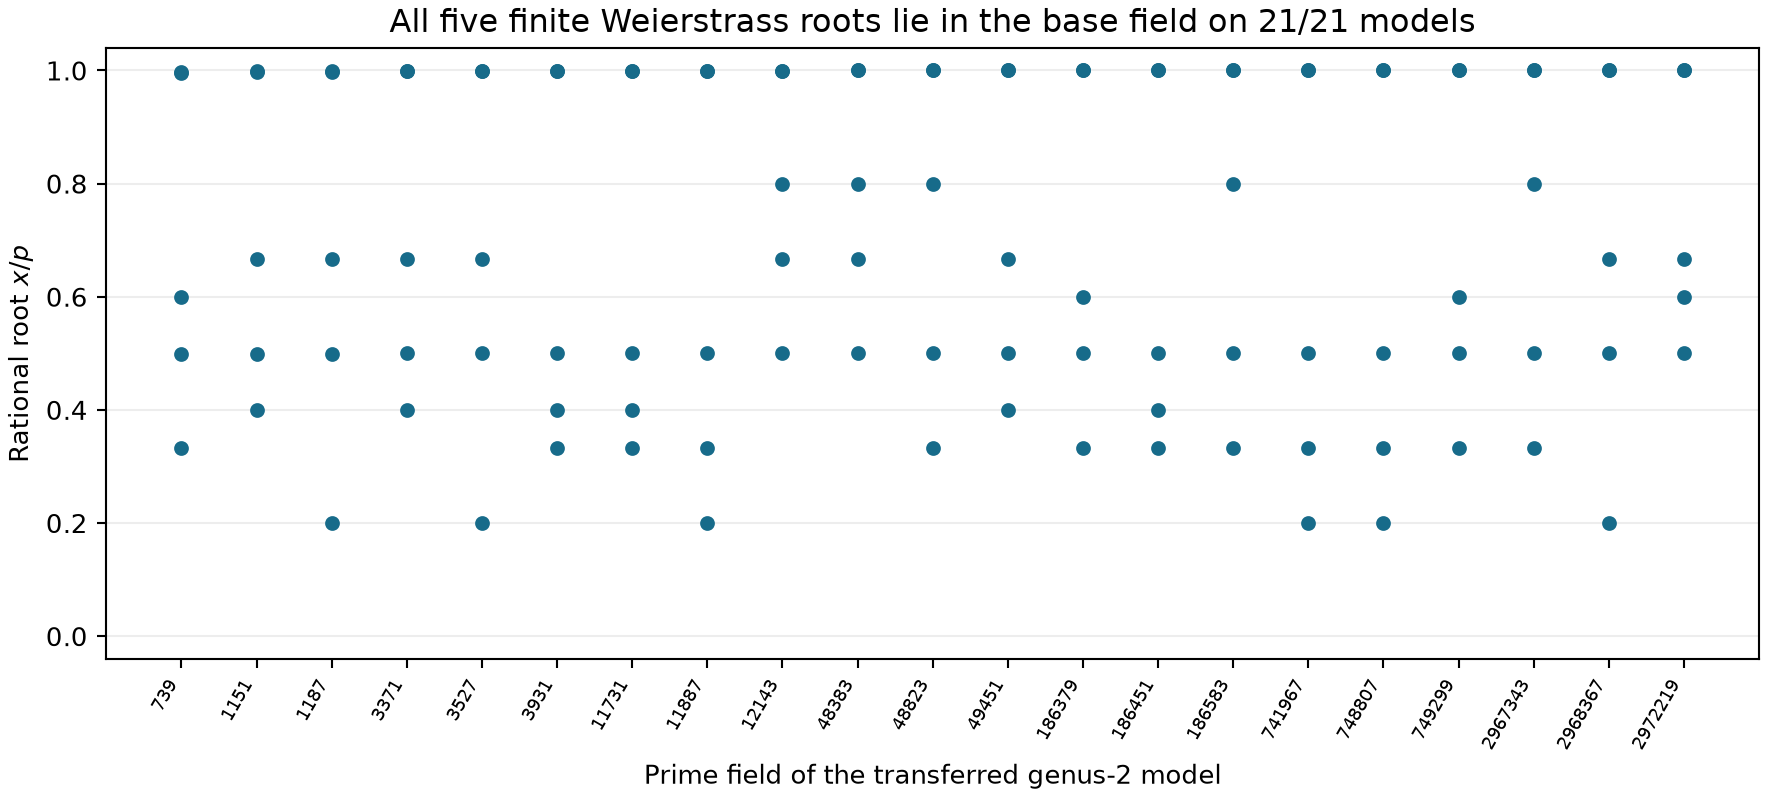
\includegraphics[width=0.98\linewidth]{kummer-model-roots.png}
\end{center}
\noindent The rational two-torsion condition addresses the field of definition
in \href{https://eprint.iacr.org/2005/314/}{Gaudry's fast-Kummer construction}.
The separate ambiguity witness shows why quotient points alone cannot supply
ordinary arbitrary-jump additions. This report does not contain a differential
walk, sign/lift-safe relation labels, or a cost ratio to rho.

\noindent Machine data: \path{results/kummer-model-gate.jsonl} and
\path{results/kummer-model-gate.replay.jsonl}.
\end{document}
